\documentclass[aspectratio=169, 9pt, t, notheorems, mathserif]{beamer}

\usepackage{polyglossia}
\setdefaultlanguage{english}

\makeatletter
\def\input@path{{../configs/}{./}} 
\makeatother

\usepackage{ctu-slides}

\usepackage{fontspec}
\usefonttheme{professionalfonts} 
\setsansfont{Technika}[
    Path = fonts/,
    Extension = .otf,
    UprightFont = *-Book,
    BoldFont = *-Bold,
    ItalicFont = *-Italic,
    BoldItalicFont = *-BoldItalic
]

\title{Automated Recognition and \\ Classification of Trading Cards} 
\subtitle{Presentation of the Unassisted project} 
\author{Jakub Adamec} 
\institute{     
    \bb{Czech Technical University in Prague}\\
    Faculty of Electrical Engineering\\
    Department of Cybernetics\\
    Visual Recognition Group
}
\date{\today}

\begin{document}

\begin{frame}[plain, noframenumbering]
    \vspace{2cm} 
    \begin{columns}[t] 
        \begin{column}{0.65\textwidth}
            {\usebeamerfont{title}\usebeamercolor[fg]{title}\huge \bb{\inserttitle}}\par
            \vspace{0.3cm}
            {\large \color{CVUTGrey}\insertsubtitle}\par
            
            \vspace{1.5cm}
            \bb{\insertauthor}\par
            \vspace{0.2cm}
            \footnotesize \insertinstitute\par
        \end{column}

        \begin{column}{0.3\textwidth}
            \raggedleft
            \vspace{-0.5cm}

            \includegraphics[width=2cm, keepaspectratio]{../configs/media/logo_CTU_vertical.pdf} 
        \end{column}
    \end{columns}
\end{frame}

\begin{frame}{Motivation and Objective}
    \bb{The problem}
    \begin{itemize}
        \item Manual sorting of trading cards (TCG) is time-consuming and prone to errors.
        \item Existing commercial solutions (e.g., CardBot) are proprietary and/or expensive. 
        \item Many different similar cards. MTG has >100k unique cards.
    \end{itemize}

    \vspace{0.5cm}
    \bb{Objective of the work}
    \begin{itemize}
        \item Software: Recognition pipeline that recognizes cards even from poor-quality photos.
        \item Hardware: Affordable and widely available components (Arduino, stepper motors...).
        \item The entire project is FOSS and well documented so that it can serve as educational material.
    \end{itemize}
\end{frame}

\begin{frame}{Recognition Pipeline}
    \begin{figure}
        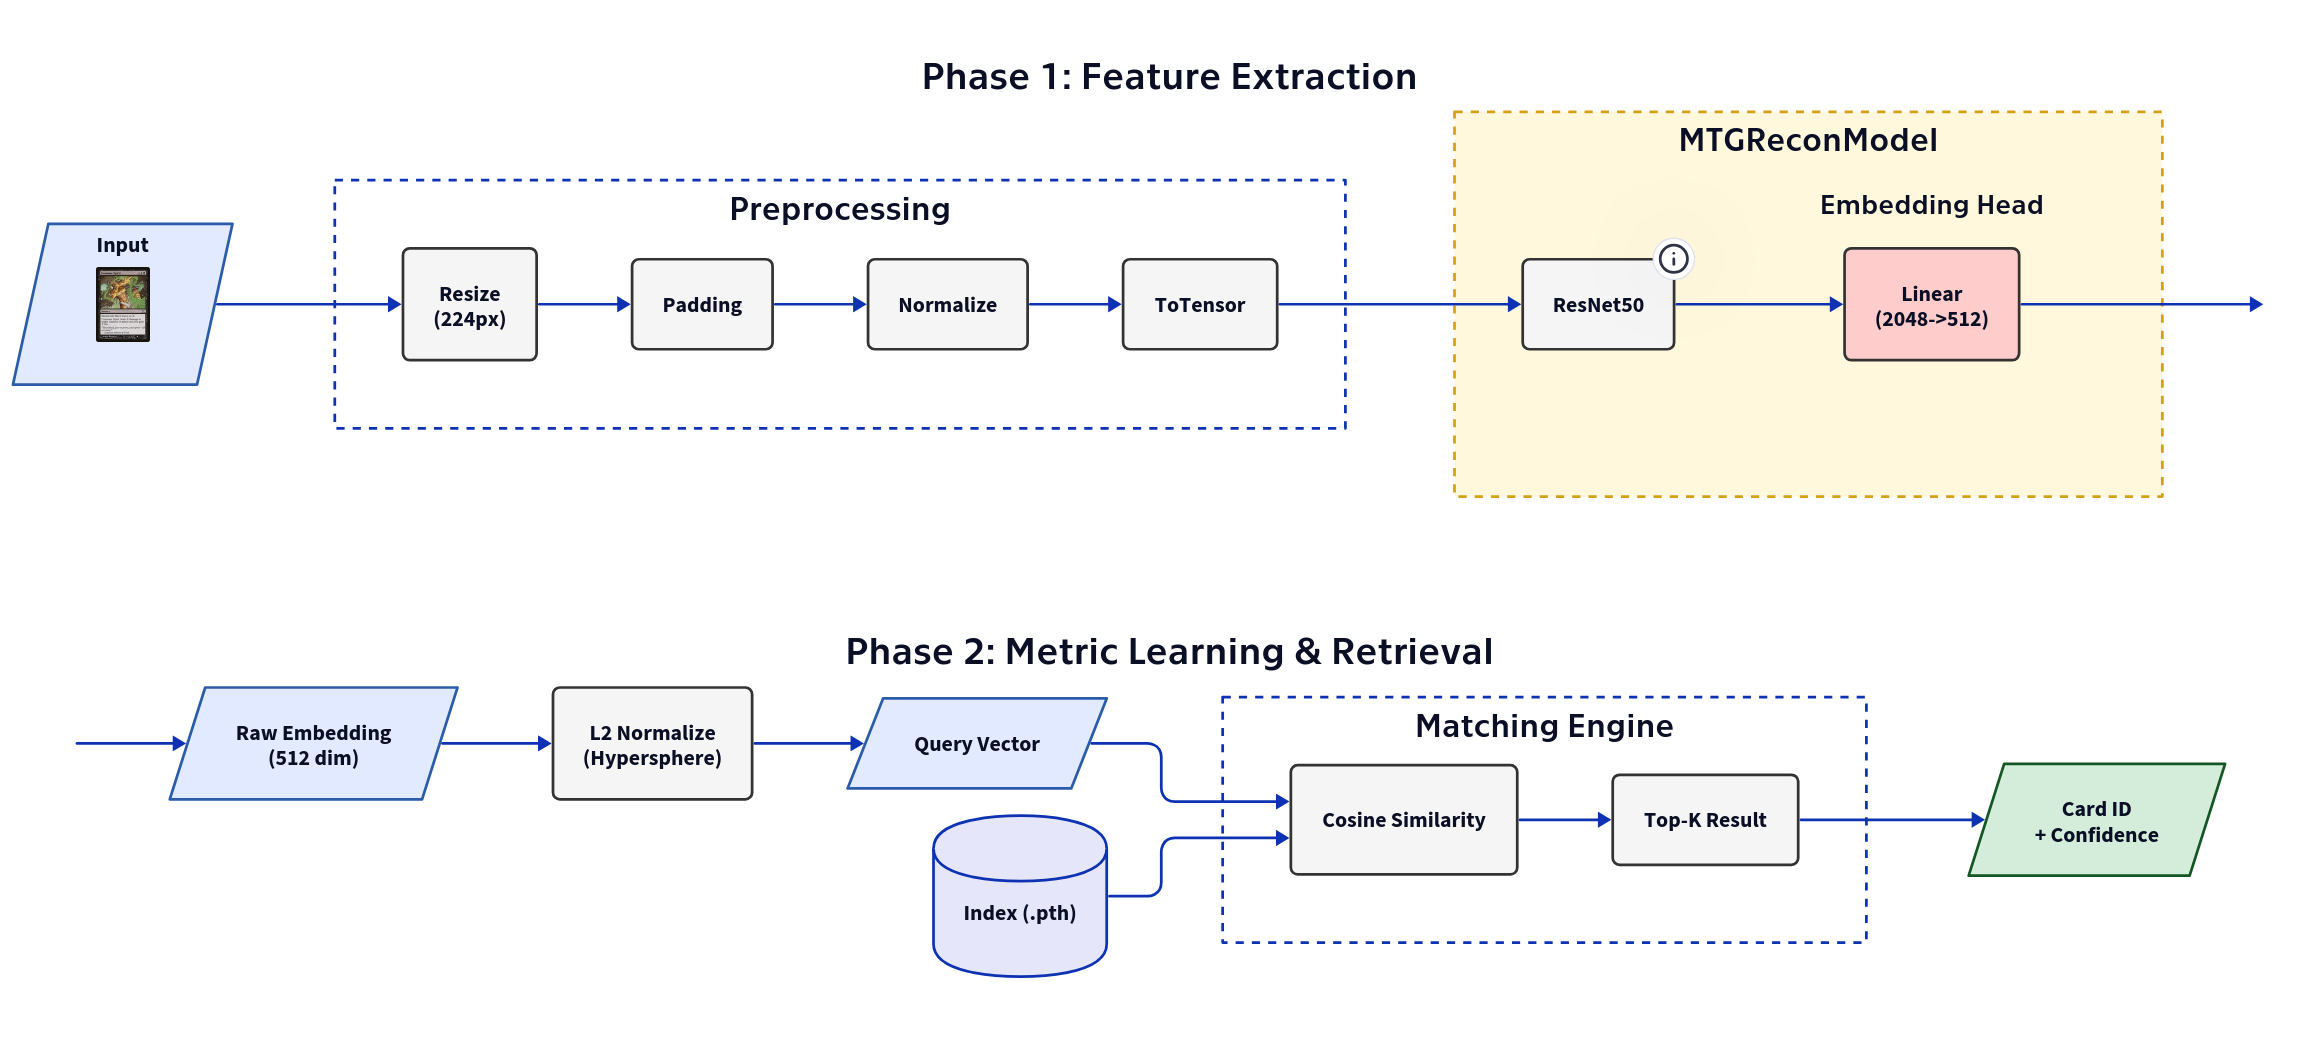
\includegraphics[scale=0.7]{../../flow.png}
    \end{figure}
\end{frame}

\end{document}
